\documentclass[a4paper,12pt,twoside,hidelinks,openright]{report}

\usepackage[spanish]{babel}
\usepackage[utf8]{inputenc}
\usepackage[usenames, dvipsnames]{color}
\usepackage{graphicx}
\usepackage{enumerate}
\usepackage{multirow}
\usepackage{graphics}
\usepackage{appendix}
\usepackage[rawfloats=true]{floatrow}
\usepackage[nottoc,numbib]{tocbibind}

\usepackage{tikz}
\usetikzlibrary{shapes,arrows}
\usepackage{subcaption}
\usepackage{amsmath,amsthm,amssymb,mathrsfs} 
\usepackage[final]{pdfpages}
\usepackage[]{placeins,flafter}
\usepackage[none]{hyphenat} \sloppy
\usepackage{xcolor}
\usepackage{adjustbox}

\usepackage{hyperref}
\hypersetup{
    colorlinks=false,
    linkcolor=blue,
    filecolor=magenta,      
    urlcolor=cyan,
    pdftitle={TFM RISC-V BNN}
    }
\urlstyle{tt} % Change url fonts to typewritter

% Coment comands
\newcommand{\javier}[1]{\textcolor{red}{#1}}
\newcommand{\dario}[1]{\textcolor{blue}{#1}}
\newcommand{\samuel}[1]{\textcolor{orange}{#1}}

% Default font to SF
\renewcommand{\familydefault}{\sfdefault}
% SF for math
\usepackage{sfmath}

%	CONFIGURACIÓN DE PÁGINA

\setlength{\paperwidth}{21cm}          % Ancho de página
\setlength{\paperheight}{29,7cm}       % Alto de página
\setlength{\textwidth}{15.5cm}         % Ancho de zona con texto
\setlength{\textheight}{24.6cm}        % Ancho de zona con texto
\setlength{\topmargin}{-1.0cm}         % Margen superior
                                      
\setlength{\oddsidemargin}{0.46cm}     % Margen izquierdo 
\setlength{\evensidemargin}{0.46cm}    

\usepackage{makeidx}
\makeindex
\index{key}
\newcommand{\myref}[1]{\color{red}\bf(\ref{#1})}

%  Custom commands
\newcommand{\todo}{\textcolor{red}{\textbf{TODO}}}
\newcommand{\boxtext}[1]{\noindent\fbox{\parbox{\textwidth}{#1}}}

\begin{document}

%%%%%%%%%%%%%%%%%%%%%%%%%%%%%%%%%%%%%%%%%%%%%%%%%%%%%%%%%%%%%%%%%%%%%%%%%%%%%%%%%%
%		PORTADA
%%%%%%%%%%%%%%%%%%%%%%%%%%%%%%%%%%%%%%%%%%%%%%%%%%%%%%%%%%%%%%%%%%%%%%%%%%%%%%%%%%

\begin{titlepage}

\vspace*{-4mm}
\begin{figure}[!h]
  \centering
	
\includegraphics[width=69.62mm]{Imagenes/UnizarLogo}
\end{figure}

\vspace*{17mm}

\fontsize{28pt}{28pt}\selectfont
\begin{center}
\setlength{\fboxsep}{3.4mm}
\adjustbox{minipage=14.4cm,cfbox=blue,center}{\begin{center} Trabajo Fin de Máster \end{center}}
\end{center}

\vspace*{5mm}


\fontsize{20pt}{20pt}\selectfont
\begin{center}
Implementación de un acelerador para redes neuronales bayesianas en plataformas RISC-V
\end{center}
\baselineskip 20pt
\begin{center}
Implementation of an acceleration unit for bayesian neural networks in RISC-V platforms
\end{center}

\vspace*{1cm} 
\baselineskip 36pt
\begin{center}
\fontsize{12pt}{12pt}\selectfont
\center{Autor}
\vspace*{3.65mm} 
\fontsize{18pt}{18pt}\selectfont
\center{Samuel Pérez Pedrajas}
\vspace*{1cm}
\baselineskip 36pt
\fontsize{12pt}{12pt}\selectfont
\center{Directores}
\vspace*{3.56mm}
\fontsize{14pt}{14pt}\selectfont
\center{Javier Resano Ezcaray}
\center{Darío Suárez Gracia}
\vspace*{1cm}
\baselineskip 36pt
\fontsize{12pt}{12pt}\selectfont
\center{Titulación}
\vspace*{3.56mm}
\fontsize{14pt}{14pt}\selectfont
\center{Máster Universitario en Ingeniería Informática}

\end{center}

\setcounter{footnote}{1}

\vspace*{16.45mm}
\fontsize{12pt}{12pt}\selectfont
\begin{center}
ESCUELA DE INGENIERÍA Y ARQUITECTURA\\
2024\\
\end{center}


\renewcommand{\thefootnote}{\arabic{footnote}}
\pagenumbering{gobble}
\end{titlepage}
\newpage

%\title{Título del trabajo final de máster}
%\author{Autor Apellido Apellido}
\pagebreak
\cleardoublepage

\baselineskip 19pt

\renewcommand{\labelitemi}{$-$}
\renewcommand{\tablename}{Tabla}

\renewcommand{\appendixname}{Anexos}
\renewcommand{\appendixtocname}{Anexos}
\renewcommand{\appendixpagename}{Anexos}


\pagenumbering{Roman}

%%%%%%%%%%%%%%%%%%%%%%%%%%%%%%%%%%%%%%%%%%%%%%%%%%%%%%%%%%%%%%%%%%%%%%%%%%%%%%%%%%%
%		Resumen
%%%%%%%%%%%%%%%%%%%%%%%%%%%%%%%%%%%%%%%%%%%%%%%%%%%%%%%%%%%%%%%%%%%%%%%%%%%%%%%%%%%

\newpage

\begin{center}
{\Large \bfseries AGRADECIMIENTOS}
\vspace{2.5cm}
\end{center}

Este trabajo ha sido parcialmente financiado por el Programa de Becas y Ayudas del Instituto de Investigación en Ingeniería de Aragón (I3A).

\newpage
\cleardoublepage
\begin{center}

\vspace{1cm}
{\Large \bfseries RESUMEN}

\vspace{2.5cm}
\end{center}

\boxtext{
\textbf{Paper abstract}\\
Neural Networks (NNs) are a very popular solution for classification tasks. As the combination of Internet of Things (IoT) with Machine Learning (ML), also known as TinyML, grows in popularity, more NN are being executed on low-end edge systems. The reliability of the predictions is crucial for safety-critical applications. Bayesian Neural Networks (BNNs) address this issue by calculating uncertainty metrics with their predictions at the cost of increasing computing requirements. This work addresses the challenges of executing BNNs inference on low-end systems. BNNs require multiple forward passes in which the weights are sampled from distributions. This sampling process can take up to 85,13\% of execution time. This work optimizes the weight sampling and integrates it within a low cost custom extension for a RISC-V CPU, improving speedup up to $\times$8,10 and similar energy savings.
}

\begin{itemize}
    \item RISC-V y extensiones
    \item Redes Bayesianas
    \item FPGA
\end{itemize}

\newpage

\cleardoublepage
\renewcommand{\contentsname}{Índice}
\tableofcontents

%%%%%%%%%%%%%%%%%%%%%%%%%%%%%%%%%%%%%%%%%%%%%%%%%%%%%%%%%%%%%%%%%%%%%%%%%%%%%%%%%%%
%		Capitulos
%%%%%%%%%%%%%%%%%%%%%%%%%%%%%%%%%%%%%%%%%%%%%%%%%%%%%%%%%%%%%%%%%%%%%%%%%%%%%%%%%%%

\chapter{Introducción}
\pagenumbering{arabic}

\section{Motivación}

\section{Objetivos y alcance}

\section{Estructura del documento}

\chapter{Estado del Arte}

Este trabajo engloba dos temas de investigación actual como son la
arquitectura RISC-V y las redes neuronales bayesianas (\textit{\textbf{B}ayesian \textbf{N}eural \textbf{N}etworks}). Este capítulo presenta un análisis del estado del arte en ambos.

\section{RISC-V}

RISC-V es una arquitectura libre de conjunto de instrucciones reducido (\textit{\textbf{R}educed \textbf{I}nstruction \textbf{S}et \textbf{C}omputer}) \cite{ricv_org}. A diferencia de las arquitecturas propietarias tradicionales, RISC-V ofrece una especificación libre, lo que permite diseñar nuevos sistemas hardware sin tener que licenciar la arquitectura.

%pagar por una licencia. Gracias a ello ha ganado un impulso e interés considerables en la industria en los últimos años \cite{riscv_survey}. Tanto es así que la Unión Europea en su proyecto \textit{European Processor Initiative} (EPI) tiene como objetivo desarrollar un procesador basado en la arquitectura RISC-V \cite{european_processor}.

RISC-V se caracteriza por su simplicidad y modularidad, esto hace que sea una buena solución para diseñar tanto procesadores de muy altas prestaciones como procesadores simples para dispositivos empotrados. El tamaño del repertorio mínimo de instrucciones de 32 bits es de 40 instrucciones, hasta el momento hay 43 extensiones no privilegiadas y 16 extensiones privilegiadas recogidas en el manual de la arquitectura \cite{riscv_scpec_unpriv, riscv_scpec_priv}.

La filosofía de diseño RISC-V consiste en partir de un conjunto de instrucciones base sencillo y extenderlo con instrucciones de dominio específico para obtener un diseño final lo mas óptimo posible pero que mantenga la flexibilidad que puede ofrecer un procesador de propósito general. Una desventaja de esta filosofía es que al adaptar un programa para utilizar diferentes extensiones su portabilidad a otros chips se reduce.

Siguiendo la filosofía de diseño RISC-V, en la actualidad empresas como Codasip \cite{codasip} o Synposis \cite{synopsis} ofrecen diseños de procesadores base junto con entornos de desarrollo para extenderlos y crear procesadores a medida para sus clientes. También existen entornos y procesadores abiertos, como Sargantana \cite{riscv_sargantana}, PULP \cite{riscv_pulp} y Rocket \cite{riscv_rocket}.

En este trabajo se ha utilizado un procesador RISC-V sencillo desarrollado anteriormente \cite{riscv_tfg}. Es un procesador de 32 bits segmentado en 5 etapas con ejecución en orden que implementa las instrucciones estándar RV32IM. RV32I indica que soporta el conjunto de instrucciones base para enteros de 32 bits. M que indica soporta el modo de ejecución \textit{Machine}, interrupciones, excepciones y la extensión Zicsr, que permite interactuar con registros de control. La Figura \ref{fig:riscv_data_pipeline} muestra un esquema simplificado de la ruta de datos del procesador. Este procesador es un ejemplo perfecto de un procesador de bajo coste y prestaciones que puede encontrarse en un sistema empotrado.

\begin{figure}[h]
    \centering
    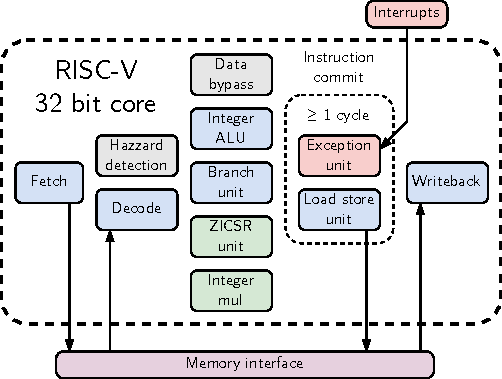
\includegraphics[width=0.9\textwidth]{Imagenes/riscv_core.pdf}
    \caption{Ruta de datos del procesador RISC-V utilizado.}
    \label{fig:riscv_data_pipeline}
\end{figure}

\section{Redes Neuronales Bayesianas}

El aprendizaje automático es una rama de la inteligencia artificial que se centra en el desarrollo de algoritmos y modelos que pueden resolver problemas para los que no han sido explícitamente programados.

Las redes neuronales (\textit{\textbf{N}eural \textbf{N}etwork}) son modelos de aprendizaje automático cuya estructura esta inspirada en el funcionamiento de redes de neuronas biológicas. Una NN esta compuesta por capas de neuronas conectadas entre si. Cada capa cuenta con un conjunto de pesos y una función de activación. Las NN necesitan un proceso de entrenamiento en el que son expuestas a un conjunto de datos etiquetados para que puedan ajustar el valor de los pesos de las diferentes capas. En los últimos años, las NN han obtenido muy buenos resultados en problemas de clasificación y regresión entre otros.

Las BNN son un tipo de NN que integran modelado probabilístico, lo que les permite cuantificar la incertidumbre en tareas de aprendizaje automático, mejorando su confianza y fiabilidad \cite{bnn_hyper_uncertainty}. Sin embargo, necesitan más parámetros para definir los pesos (normalmente el doble que una NN convencional) y la inferencia es más compleja. Los pesos de las BNN son distribuciones de probabilidad, normalmente distribuciones gaussianas, que se han de muestrear durante las propagaciones de la entrada. El algoritmo de inferencia más común para las BNN requiere múltiples propagaciones de la entrada de la red, aumentando drásticamente el coste computacional del mismo \cite{bnn_theory_paper}. 

La Figura \ref{fig:bnn_vs_nn_example} muestra la utilidad de las métricas de incertidumbre con un ejemplo simple. Considerando una NN convencional y una BNN ambas entrenadas para clasificar imágenes de perros y gatos, en el caso de que se les pidiera clasificar un dato anómalo, como la imagen de un tigre, con la BNN se obtendría un valor de incertidumbre alto, indicando una anomalía en la predicción, mientras que con una NN convencional no se tendría ningún indicio de que el dato de entrada era anómalo.

\begin{figure}[h]
    \centering
    \includegraphics[width=\textwidth]{Imagenes/nn_bnn_example.pdf}
    \caption{Ejemplo sencillo de utilidad de las métricas de incertidumbre aportadas por las BNN. Una NN convencional y una BNN, ambas entrenadas para clasificar imágenes de perros y gatos, reciben como entrada la imagen de un tigre. La BNN es capaz de detectar el dato anómalo mientras que la NN convencional no.}
    \label{fig:bnn_vs_nn_example}
\end{figure}

La Figura \ref{fig:neuron_comparation} muestra una comparación sencilla de una neurona clásica y de una neurona bayesiana, ambas con una función de activación de rectificación (\textit{\textbf{Re}ctified \textbf{L}inear \textbf{U}nit}).

% Vertically alling two sufigures and keep subcaption using floatrow and subcaptions pkgs
\begin{figure}[htb]
  \floatsetup{heightadjust=all, valign=c}
  \begin{subcaptiongroup}
  \begin{floatrow}
    \ffigbox{%
      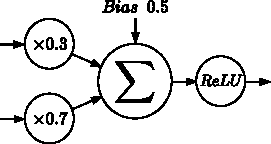
\includegraphics[width=0.48\textwidth]{Imagenes/clasic_neuron.pdf}
    }{%
      \caption{Neurona clásica}%
      \label{fig:clasic_neuron}%
    }
    \ffigbox{%
      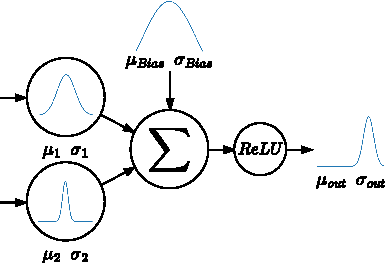
\includegraphics[width=0.49\textwidth]{Imagenes/bnn_neuron.pdf}
    }{%
      \caption{Neurona bayesiana}%
      \label{fig:bnn_neuron}%
    }
  \end{floatrow}
  \end{subcaptiongroup}
  \caption{Comparación de una neurona clásica con respecto a una neurona bayesiana, ambas con la misma función de activación ReLU. Los pesos de la neurona convencional son valores estáticos mientras que los de la neurona bayesiana son distribuciones gaussianas parametrizadas mediante medias y desviaciones típicas.}%
  \label{fig:neuron_comparation}%
\end{figure}

En un entorno de internet de las cosas (\textit{\textbf{I}nternet \textbf{o}f \textbf{T}hings}) donde los datos pueden ser incompletos o ruidosos la capacidad de cuantificar la incertidumbre es crucial para tomar decisiones confiables en aplicaciones críticas. Por lo que las BNN son una muy buena herramienta para mejorar la precisión y la robustez de los sistemas de aprendizaje automático en estos entornos.

Las métricas de incertidumbre proporcionadas por las BNN son muy útiles para detectar diferentes tipos de situaciones. Por ejemplo, pueden servir para valorar la confianza de la predicción, si una predicción tiene una alta incertidumbre podría indicar que es menos confiable y que requeriría de verificación humana. También pueden utilizarse para valorar la calidad los datos de entrenamiento, si los datos de entrenamiento contienen muestras mal etiquetadas sus predicciones tendrán una mayor incertidumbre asociada. Alcolea \emph{et al.} \cite{bnn_hyper_uncertainty} \javier{ mostraron que existe una clara correlacción entre la incertidumbre y la precisión en un modelo bien entrenado, por tanto la incertidumbre se puede utilizar para identificar salidas con menor probabilidad de acierto de la requerida.} También observaron que al entrenar una BNN con los datos de 2 clases mezclados se aprecia un claro incremento en la incertidumbre de las predicciones asociadas a esas clases, y que \javier{la incertidumbre aumentaba cuando se añadía ruido aleatoria a las entradas}. Otro posible uso es detectar que los datos de entrenamiento no reflejan correctamente la realidad, predicciones con alta incertidumbre pueden indicar que los datos que esta procesando el modelo no se parecen a los datos con los que ha sido entrenado. En entornos dinámicos como IoT, donde las condiciones pueden cambiar rápidamente, si la incertidumbre en las predicciones aumenta repentinamente, puede indicar un cambio en el entorno que requiera una recalibración del modelo.

\subsection{Marco teórico} \label{sec:bnn_formulas}

Estas redes neuronales utilizan el Teorema de Bayes,  ecuación \ref{eq:bayes_theo}, para modelar la probabilidad de un conjunto de pesos $w$ dado un conjunto de datos de entrenamiento $D = \{x, y\}$. Esta distribución de probabilidad es la probabilidad a posteriori.
\begin{equation} \label{eq:bayes_theo}
p(w|D) = \dfrac{p(D|w) p(w)}{p(D)}
\end{equation}

El entrenamiento de una BNN consiste en calcular esta distribución a posteriori. Calcular esta distribución para un modelo grande y complicado como una BNN es intratable. Para aproximar esta distribución se utilizan métodos inferencia bayesiana. El método más común es la inferencia variacional, que aproxima la distribución a posteriori usando una más simple $q_{\phi}(w)$. Esta aproximación se realiza minimizando la divergencia de Kullback-Leibler \cite{kl_divergence} entre $q_{\phi}(w)$ y $p(w|D)$ mediante la actualización de un conjunto de parámetros $\phi$. Teóricamente, las distribuciones podrían tener cualquier forma, pero para reducir el espacio de búsqueda solo se utilizan distribuciones simétricas y simples. Las distribuciones gaussianas son una buena opción porque solo se definen con dos parámetros, lo que ayuda a reducir el tamaño del modelo.

En consecuencia, una BNN entrenada consiste en un conjunto de medias y desviaciones de diferentes distribuciones gaussianas $\phi = \{\mu, \sigma\}$, lo que significa que los pesos se convierten en distribuciones de probabilidad en lugar de valores fijos, y la salida también se convierte en una distribución en lugar de un valor único. Esto permite medir la incertidumbre de la predicción. La Ecuación \ref{eq:bayes_inference} muestra la distribución de predicción a posteriori de una nueva observación $x^*$.
\begin{equation} \label{eq:bayes_inference}
p(y^*|x^*,D) = \int p(y|x^*,w) p(w|D) dw
\end{equation}

Mediante métodos de Monte Carlo se puede aproximar la integral de la Ecuación \ref{eq:bayes_inference}. En este caso, las muestras son diferentes propagaciones estocásticas de la entrada. En cada una de estas propagaciones, los pesos se muestrean de las distribuciones gaussianas que forman la distribución a posteriori aproximada.

Siendo $T$ el número de muestras, $K$ el número de clases posibles y una muestra $a_t = p(y^* = c_k | x^*, w_t)$. Cada muestra $a_t$ es un vector de longitud $K$, cada uno de sus componentes $c_k$ representa la probabilidad de clasificar $x^*$ como $y^*$. Para obtener una única predicción se puede tomar el máximo $c_k$ del vector promedio de todas las muestras.

\subsubsection{Cálculo de la incertidumbre}

En problemas de clasificación, se puede medir la incertidumbre de una predicción utilizando las diferentes muestras Monte Carlo obtenidas \cite{uncertainty_metrics}. A continuación se explica como obtener las métricas mas relevantes y lo que representan.

La incertidumbre predictiva ($\mathbb{H}$) representa la incertidumbre de una predicción en el rango $[0, \log(K)]$ y puede calcularse utilizando la Ecuación \ref{eq:predictive_uncertainty}.
\begin{equation} \label{eq:predictive_uncertainty}
\mathbb{H}(y|x,D) = - \sum^K_{k=1} \left[ \left( \dfrac{1}{T} \sum^T_{t=1} a_t \right) \log\left( \dfrac{1}{T} \sum^T_{t=1} a_t \right) \right]
\end{equation}

La incertidumbre puede dividirse en dos, aleatoria y epistémica, $\mathbb{H}$ captura ambas. La entropía esperada ($\mathbb{E}p$) captura la incertidumbre aleatoria, que es causada por ambigüedades en el conjunto de datos como mediciones ruidosas, clases superpuestas o muestras mal etiquetadas. $\mathbb{E}p$ puede calcularse utilizando la Ecuación \ref{eq:expected_entropy}.
\begin{equation} \label{eq:expected_entropy}
\mathbb{E}{p(w|D)}[\mathbb{H}(y|x,D)] = \dfrac{1}{T} \sum^T{t=1} \left( -\sum^K_{k=1} a_{t} \log(a_t) \right)
\end{equation}

La incertidumbre epistémica representa lo que el modelo no sabe debido a la falta de datos durante el proceso de entrenamiento, y puede calcularse utilizando la información mutua (\textit{\textbf{M}utual \textbf{I}nformation}) mostrada en la Ecuación \ref{eq:mutual_information}.
\begin{equation} \label{eq:mutual_information}
MI(y,w|x,D) = \mathbb{H}(y|x,D) - \mathbb{E}_{p(w|D)}[\mathbb{H}(y|x,D)]
\end{equation}

\subsection{Aceleración hardware}

La aceleración de algoritmos de aprendizaje automático es un campo de investigación muy activo con muchas propuestas recientes \cite{survey_ai22}. La aceleración de las BNN no es una excepción, debido en parte al elevado coste de su algoritmo de inferencia. Otros trabajos se han centrado en desarrollar aceleradores de alto rendimiento para el proceso completo de inferencia \cite{bnn_grng_accel, sampling_free_bnn_accel, bnn_clt_approx}.

Awano \emph{et al.} propusieron un acelerador sin múltiples propagaciones ni muestreo para el algoritmo de inferencia de las BNN, reemplazando la función de activación ReLU por una función cuadrática \cite{sampling_free_bnn_accel}. Su trabajo muestra buenos resultados para el conjunto de datos MNIST, pero otros trabajos han demostrado que este enfoque no es generalizable y no funciona bien con otros modelos \cite{bnn_clt_approx}. Por esta razón, este trabajo se centra en el algoritmo de múltiples propagaciones con muestreo, ya que es el método más estándar y ha sido ampliamente demostrado que da buenos resultados para varios diferentes conjuntos de datos \cite{bnn_grng_accel, bnn_clt_approx, bnn_hyper_uncertainty}.

El muestreo de distribuciones para generar los pesos es una parte fundamental de los trabajos que siguen el enfoque de múltiples propagaciones. Cai \emph{et al.} propusieron un acelerador de inferencia de BNN con 2 posibles generadores de números aleatorios gaussianos (\textit{\textbf{G}aussian \textbf{R}andom \textbf{N}umber \textbf{G}enerator}) \cite{bnn_grng_accel}. Uno basado en el teorema central del límite (TCL) utilizando la distribución binomial y otro en el método de Wallace \cite{wallace_grng}.

Los GRNG son un tema que ya ha sido explorado en profundidad \cite{grng_survey}. Trabajos anteriores han mostrado que los GRNG basados en el CLT no muestran una precisión elevada en la cola de la distribución \cite{clt_grng}. Sin embargo, en el caso de la inferencia de las BNN no es necesario tener un GNRG preciso. Hirayama \emph{et al.} demostraron que utilizando un GRNG de poca precisión basado en una \textit{Lookup Table} (LUT) se obtienen buenos resultados \cite{bnn_lut_grng}.

En otro trabajo Awano \emph{et al.} diseñaron un acelerador que aproximan la salida final del modelo utilizando generadores hardware de muestras Bernoulli \cite{bnn_clt_approx}, bajo la condición de que el TCL podría aplicarse al modelo en general. La Figura \ref{fig:b2n2_clt} muestra un diagrama de su aproximación.

\begin{figure}[h]
    \centering
    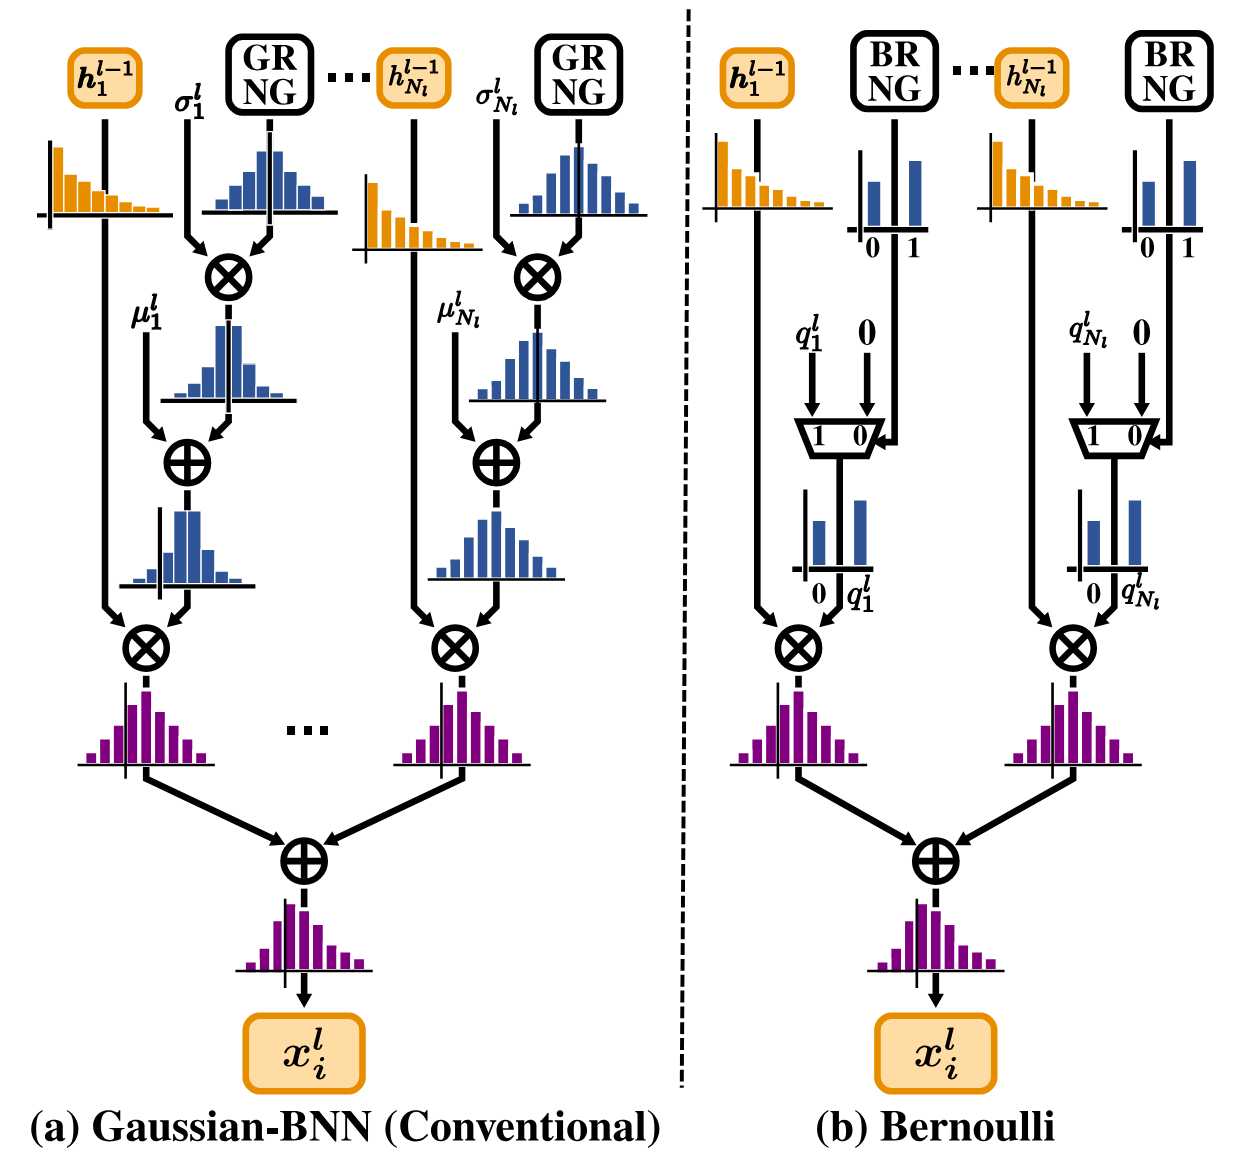
\includegraphics[width=0.55\textwidth]{Imagenes/b2n2_clt.png}
    \caption{Comparación de muestrear distribuciones gaussianas o distribuciones de Bernoulli en una BNN. Debido al TCL la distribución final es independiente de las distribuciones muestreadas \cite{bnn_clt_approx}.}
    \label{fig:b2n2_clt}
\end{figure}

Una ventaja clave de los generadores de muestras Bernoulli radica en su implementación en hardware. A diferencia de los métodos de software que dependen de operaciones de salto, que pueden degradar el rendimiento de las CPU modernas, los generadores hardware pueden implementarse utilizando componentes simples como comparadores y multiplexores, lo que los hace de bajo coste y eficientes.

\subsection{Soporte de bibliotecas}

Este trabajo tiene como objetivo ejecutar inferencia de estas redes en entornos RISC-V de bajas prestaciones, donde actualmente no existe un conjunto de bibliotecas que lo permita. TensorFlow Probability \cite{tfprob} permite entrenar y ejecutar inferencia de BNN utilizando precisión en punto flotante. Por otro lado, en el caso de PyTorch, existe BayesianTorch desarrollado por IntelLabs \cite{bayesian_torch}, que ofrece la misma funcionalidad.

TensorFlowLite \cite{tflite} es la versión de TensorFlow diseñada para sistemas empotrados, ofrece funcionalidades como la cuantización de modelos y la inferencia utilizando precisión de enteros para las NN convencionales. Sin embargo, aun no soporta BNN. En una actualización reciente, BayesianTorch ha añadido soporte para la cuantización de BNN \cite{bnn_quant}. Este trabajo se centra en el ecosistema de Tensorflow debido a que se han utilizado modelos desarrollados dicho entorno para su validación. 

\chapter{Redes Neuronales Bayesianas en RISC-V}

En esta sección se explican los pasos y bibliotecas desarrolladas para poder ejecutar inferencia de BNN de manera eficiente en un procesador RISC-V con solo soporte para precisión entera. La Figura \ref{fig:experiment_pipeline} muestra el proceso y componentes necesarios.

\begin{figure}[h]
    \centering
    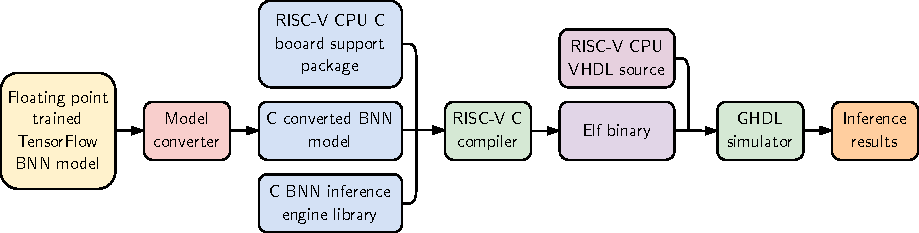
\includegraphics[width=\textwidth]{Imagenes/experiment_pipeline.pdf}
    \caption{\todo}
    \label{fig:experiment_pipeline}
\end{figure}

\section{Componentes desarrollados}

Para poder llevar a cabo el proceso de la Figura \ref{fig:experiment_pipeline} se han realizado las siguientes tareas: desarrollar un conversor de modelos, desarrollar un motor de inferencia de BNN, actualizar el \textit{\textbf{B}oard \textbf{S}upport \textbf{P}ackage} (BSP) del procesador y desarrollar una herramienta de análisis de resultados.

\subsection{Conversor de modelos}

Se ha desarrollado una herramienta en Python que convierte modelos BNN TensorFlow ya entrenados en precisión de punto flotante a ficheros de código C que puedan ejecutarse junto al motor de inferencia explicado en la Sección \ref{sec:motor_inferencia_c}. Esta herramienta realiza las siguientes tareas:

\begin{itemize}
    \item Transformar los pesos a coma fija. Coma fija es un formato que permite representar y operar con números decimales utilizando hardware de precisión entera.
    \item Analizar la precisión mínima necesaria. Buscar el tamaño de dato más pequeño en los que los pesos transformados se puedan almacenar. \todo
    \item Generar vectores de pesos. Generar código C que almacene los pesos en vectores aplanados.
    \item Generar función de inferencia. Analizar que capas forman el modelo y generar el código de una función de inferencia utilizando las funciones proveídas por el motor.
    \item Transformar los datos de prueba a coma fija.
    \item Generar vector de datos de prueba.
\end{itemize}

\subsection{Actualización del Board Support Package}

Con el objetivo de mejorar la experiencia de desarrollo del motor de inferencia se actualizó el BSP del procesador para dar soporte a la biblioteca estándar C (libc) y algunas funcionalidades de C++. De esta forma se pueden utilizar funciones útiles de libc cómo \texttt{printf}, o \texttt{memset} entre otras. Para ello se actualizaron las herramientas y ficheros de compilación, se añadieron funciones \textit{stub} para las llamadas al sistema no implementadas y se implementaron versiones modificadas de \texttt{\_write} y \texttt{\_exit}.

\subsection{Motor de inferencia} \label{sec:motor_inferencia_c}

Se ha desarrollado una librería de funciones que ejecutan la inferencia de capas BNN estándar y convolucionales con funciones de activación ReLU o exponenciales normalizadas (SoftMax) utilizando precisión de punto fijo. Mientras que calcular la función ReLU es trivial la función SoftMax no. Dicha función toma un vector de componentes $x \in X$ de tamaño $N$ como entrada y devuelve otro del mismo tamaño cuyos componentes $y\in Y$ se calculan según la Ecuación \ref{eq:softmax}.
\begin{equation} \label{eq:softmax}
y_i = \dfrac{e^{x_i}}{\sum_{j = 0}^N e^{x_j}}
\end{equation}

Para calcular esta función utilizando coma fija es necesario calcular la función exponencial en dicho formato. Para evitar desbordamientos de la función exponencial se va a utilizar la función SoftMax equivalente mostrada en la Ecuación \ref{eq:softmax_neg}.
\begin{equation} \label{eq:softmax_neg}
y_i = \dfrac{e^{x_i - \max(X)}}{\sum_{j = 0}^N e^{x_j - \max(X)}}
\end{equation}

En esta versión de la función se cumple que $x_i \in (-\infty, 0]$ por lo que $e^{x_i} \in (0,1]$. Para calcular la función exponencial se va a utilizar la Ecuación \ref{eq:split_exp}, dividiendo la entrada $x_i$ en su parte entera $a_i$ y su parte decimal $b_i$.
\begin{equation} \label{eq:split_exp}
e^{x_i} = e^{a_i+b_i} = e^{a_i} e^{b_i}
\end{equation}

La parte entera $e^{a_i}$ se calcula mediante una LUT de 20 entradas para el rango $[e^{-19}, e^{0}]$. A partir de $e^{-19}$ los valores son demasiado pequeños como para representarlos con la precisión disponible por lo que siempre valen $0$. La parte decimal $e^{b_i}$ se aproxima mediante los 8 primeros términos de la serie de Taylor mostrada en la Ecuación \ref{eq:exp_taylor}. Para optimizar y evitar las divisiones los valores de $\dfrac{1}{n!}$ para $n \in [2,7]$ se han almacenado en una LUT.
\begin{equation} \label{eq:exp_taylor}
e^{b_i} \approx \sum_{n=0}^{7} \dfrac{{b_i}^n}{n!}
\end{equation}

Como se ha explicado previamente, las BNN necesitan muestrear distribuciones gaussianas. Como método de muestreo base se utilizada un algoritmo basado en la suma de distribuciones uniformes, dicha suma se aproximan a una distribución gaussiana debido al TCL, mostrado en la Ecuación \ref{eq:tcl_unif}.
\begin{equation} \label{eq:tcl_unif}
\sum_{n=0}^{N} \mathcal{U}_n(0,1) \sim \mathcal{N} \left( \dfrac{N}{2}, \sqrt{\dfrac{N}{12}} \right)
\end{equation}

El algoritmo implementado genera muestras de $\mathcal{N}(0,1)$ para luego transformarlas en muestras de una distribución gaussiana arbitraria $\mathcal{N}(\mu, \sigma)$ de media $\mu$ y desviación típica $\sigma$ utilizando la Ecuación \ref{eq:gauss_linear}.
\begin{equation} \label{eq:gauss_linear}
\mathcal{N}(\mu, \sigma) = \sigma \mathcal{N}(0,1) + \mu
\end{equation}

Para ello utiliza la suma de 12 distribuciones uniformes y posteriormente centra la distribución como muestra la Ecuación \ref{eq:tcl_12center}.
\begin{equation} \label{eq:tcl_12center}
\sum_{n=0}^{12} \mathcal{U}_n(0,1) - 6 \sim \mathcal{N}(0,1)
\end{equation}

Para generar muestras de distribuciones uniformes se utiliza una versión del algoritmo Xorshift de 32 bits \cite{xorshift}. Es un algoritmo sencillo para generar números pseudoaleatorios solamente con instrucciones \texttt{xor} y \texttt{shift}.

Para calcular las métricas de incertidumbre se necesita la función logaritmo por lo que se ha implementado una versión del algoritmo desarrollado por Turner \cite{binary_log} para calcular el logaritmo de un número en coma fija. 

\subsection{Verificación automática}

Para analizar el correcto funcionamiento del motor de inferencia y estudiar el impacto en el rendimiento de las optimizaciones posteriores se ha desarrollado una herramienta que compara las predicciones del conjunto de datos de prueba obtenidas con el motor de inferencia y TensorFlow.

Para comparar los conjuntos de predicciones se han utilizado la métrica de precisión y las métricas de incertidumbre. La precisión es simplemente el ratio de predicciones correctas sobre el número de predicciones. Analizar las métricas de incertidumbre es más complejo, por lo que se han utilizado los siguientes gráficos para ello.\\



\boxtext{
\begin{itemize}
    \item \todo
    \item incertidumbre media de cada clase
    \item histograma de las predicciones correctas, incorrectas
    \item recta calibración
    \item precisión por grupos
    \item cambio de prueba
    \item cambio de prueba A
\end{itemize}
}

\section{Análisis de la carga de trabajo}



\section{Optimizaciones software}


\chapter{Extendiendo RISC-V}

\section{Diseño del acelerador}

\subsection{Generación de números pseudoaleatorios}

\begin{figure}[h]
    \centering
    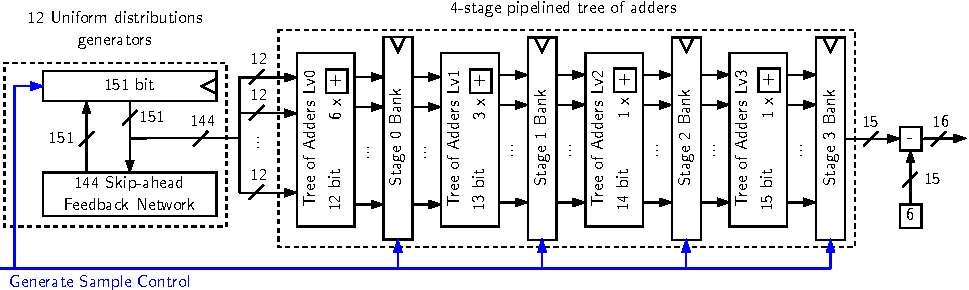
\includegraphics[width=\textwidth]{Imagenes/grng.pdf}
    \caption{\todo}
    \label{fig:aa}
\end{figure}

\section{Modificaciones al procesador}

\begin{figure}[h]
    \centering
    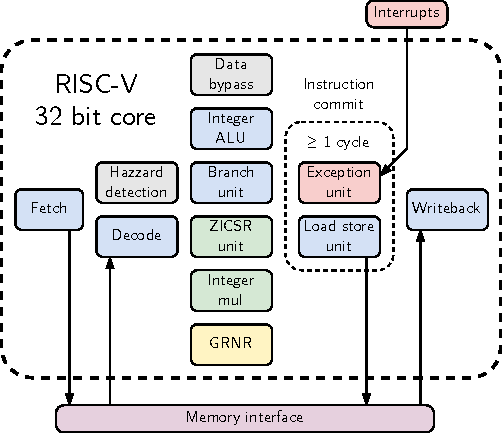
\includegraphics[width=0.9\textwidth]{Imagenes/riscv_core_extended.pdf}
    \caption{\todo}
    \label{fig:bb}
\end{figure}


\subsection{Actualizar el compilador}

\section{Análisis de resultados}

\subsection{Análisis de coste}

\chapter{Conclusiones}


%%%%%%%%%%%%%%%%%%%%%%%%%%%%%%%%%%%%%%%%%%%%%%%%%%%%%%%%%%%%%%%%%%%%%%%%%%%%%%%%%%%
%		BIBLIOGRAFÍA Y REFERENCIAS
%%%%%%%%%%%%%%%%%%%%%%%%%%%%%%%%%%%%%%%%%%%%%%%%%%%%%%%%%%%%%%%%%%%%%%%%%%%%%%%%%%%

\bibliographystyle{unsrt} %plaindin
\bibliography{Bibliografia_TFM}
\nocite{*} 

\newpage
\renewcommand\listfigurename{Lista de Figuras}
\listoffigures

\newpage
\renewcommand\listtablename{Lista de Tablas}
\listoftables

%%%%%%%%%%%%%%%%%%%%%%%%%%%%%%%%%%%%%%%%%%%%%%%%%%%%%%%%%%%%%%%%%%%%%%%%%%%%%%%%%%%
%		ANEXOS
%%%%%%%%%%%%%%%%%%%%%%%%%%%%%%%%%%%%%%%%%%%%%%%%%%%%%%%%%%%%%%%%%%%%%%%%%%%%%%%%%%%

\newpage
\appendix
\clearpage
\addappheadtotoc
\appendixpage
\chapter{Un anexo}


Sed ut perspiciatis unde omnis iste natus error sit voluptatem accusantium doloremque laudantium, totam rem aperiam, eaque ipsa quae ab illo inventore veritatis et quasi architecto beatae vitae dicta sunt explicabo. Nemo enim ipsam voluptatem quia voluptas sit aspernatur aut odit aut fugit, sed quia consequuntur magni dolores eos qui ratione voluptatem sequi nesciunt. Neque porro quisquam est, qui dolorem ipsum quia dolor sit amet, consectetur, adipisci velit, sed quia non numquam eius modi tempora incidunt ut labore et dolore magnam aliquam quaerat voluptatem. Ut enim ad minima veniam, quis nostrum exercitationem ullam corporis suscipit laboriosam, nisi ut aliquid ex ea commodi consequatur? Quis autem vel eum iure reprehenderit qui in ea voluptate velit esse quam nihil molestiae consequatur, vel illum qui dolorem eum fugiat quo voluptas nulla pariatur? At vero eos et accusamus et iusto odio dignissimos ducimus qui blanditiis praesentium voluptatum deleniti atque corrupti quos dolores et quas molestias excepturi sint occaecati cupiditate non provident, similique sunt in culpa qui officia deserunt mollitia animi, id est laborum et dolorum fuga. Et harum quidem rerum facilis est et expedita distinctio. Nam libero tempore, cum soluta nobis est eligendi optio cumque nihil impedit quo minus id quod maxime placeat facere








%%%%%%%%%%%%%%%%%%%%%%%%%%%%%%%%%%%%%%%%%%%%%%%%%%%%%%%%%%%%%%%%%%%%%%%%%%%%%%%%%%%


\end{document}